\chapter{\TheSolutionName{}}
\label{cap:proposal}

In this chapter, we propose the \TheSolutionName{}, a solution for offloading some of Zeek's operations discussed in Section \ref{sec:candidate_operations} to Network Programmable Forwarding Devices compatible with P4. This proposal uses the Reconfigurable Network Analytics (RNA) architecture, which was initially proposed by Ilha \cite{Ilha2022}. Since \TheSolutionName{} also contributed to RNA's development, this text describes and presents them together.

\begin{figure}[h]
    \caption{RNA Framework - High-level architectural view}
    \begin{center}
        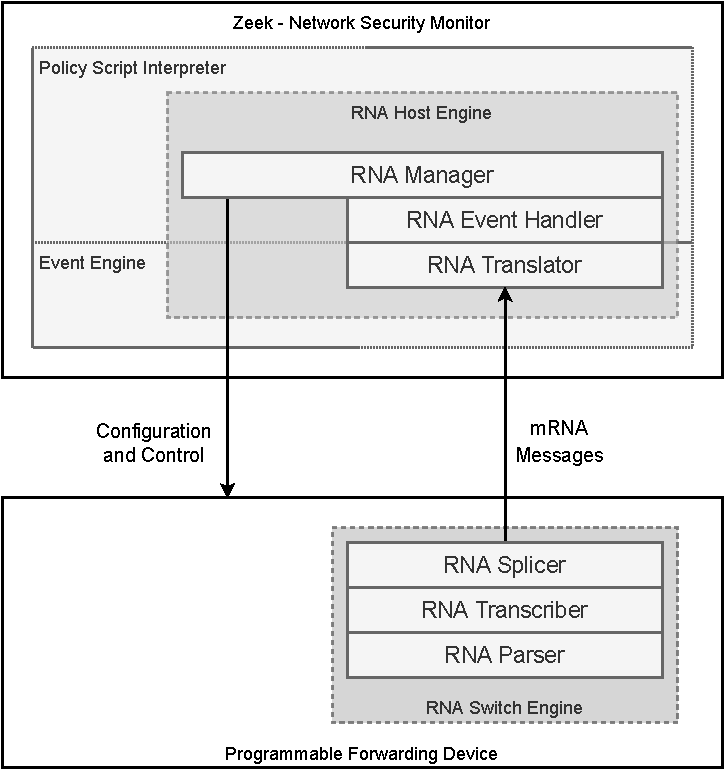
\includegraphics[width=0.7\textwidth]{images/arch_high_level.pdf}  
    \end{center}
    \label{fig:arch_high_level}
    \legend{Source: the author, adapted from Ilha \cite{Ilha2022}}
\end{figure}

Figure \ref{fig:arch_high_level} illustrates the RNA architecture. It is composed of two high-level components: the RNA Host Engine, which executes in one of Zeek's work nodes inside the IDS; and the RNA Switch Engine, which is executed in a P4 switch. Both components work together to offload packet analysis from Zeek to a programmable forwarding device. The RNA Switch Engine is able to better parse packets and identify some of their characteristics, which are then summarized and sent to the RNA Host Engine. This summarized message is called mRNA. When the IDS receives this message, it is first processed by our Host Engine. It then converts the summarized message into Zeek's native structures, which can then be forwarded to Zeek's normal processing pipeline. This procedure allows us to bypass some operations that would be costly, and deliver this information one step closer to the Policy Script Interpreter (PSI, Section \ref{sec:zeek_psi}), without disturbing its flow. By doing so, we make it that no change is required on existing scripts running on the PSI.

% TODO: check what to call this "'custom software' to be executed both...."
In the original concept of RNA, depending on the IDS scripts chosen to be monitored by the operator, it is necessary to develop custom software to be executed both by the Host Engine and the Switch Engine. This ad-hoc development process quickly becomes impractical when we increase the number of desired scripts to be offloaded. For this reason, later propose an automatic code generation tool, which allows \TheSolutionName{} to be a modular solution, where new offloaded scripts can be added or removed, without the need to develop new software. Before detailing this automated process, first, we revisit the architectural concepts.

% ==============================================================================
%                               RNA OVERVIEW
% ==============================================================================
\section{Overview}

In this section, we'll describe the components shown in Figure \ref{fig:arch_high_level}. We start with the RNA Host Engine, since it is the controlling part of the whole deployment, and then we describe the RNA Switch Engine.


% TODO: check if we'll remove the "RNA Event Handler" completely, or say it was removed but exists in the original RNA
The \textbf{Host Engine} unfolds into three components. The \textbf{RNA Manager} is a Zeek Script, which first configures the P4 switch, setting up a monitoring session and loading all P4 code that is required to execute the offloaded tasks. After configuring the switch, it registers all RNA Translators (one per-protocol of interest), so they receive mRNA messages. The \textbf{Translators} wait for such messages and translate them to Zeek native structures. Those structures are then used to trigger events, which are then consumed by the running scripts.

% % Removed: too much 'unwanted' information
% In order not to override and disturb the existing Zeek Packet and Protocol Analyzers described in Section \ref{sec:packet_analysis_framework}, the Translators are registered using a different protocol, the RNA protocol, which is used by the mRNA message (Section \ref{sec:mrna_message}) and is built over Ethernet. This means the packets encoded as mRNA messages, even if they represent an ICMP event, for example, will be first analyzed by the Ethernet \textit{Analyzer}, then the RNA Translator \textit{Analyzer}, where the normal flow for an ICMP packet would be the following analyzers: Ethernet, IPv4, and ICMP.

The \textbf{RNA Switch Engine} is the program that executes in our P4-compatible programmable forwarding device. It has three components and we'll be following the route of an incoming packet to explain them. The first component that processes a packet is the \textbf{RNA Parser}. It parses and extracts headers from each protocol, from the link layer, up to the application layer if required. After all headers have been extracted, the packet enters P4's ingress pipeline, where the \textbf{RNA Transcriber} is executed. It extracts useful information from the packet and sets metadata that later will be used to build our summarized message, while also filtering some undesired packets. Having all the required metadata and going into P4's egress pipeline, the \textbf{RNA Splicer} builds and sends our summarized message, the mRNA, to the Host Engine with all information it may require to trigger a native Zeek Event.

Another important structure to be explained is The \textbf{mRNA Message} is a summary of a packet, summarizing all the information that the Switch Engine was able to extract from it. Sending an mRNA message is better than sending the whole packet because the original packet contains a lot of headers that still would need to be parsed, a lot of information that is not necessary in some cases, and is not validated. In the summarized message, all information from L2 up to the L7 layer is gathered, filtered, and even formatted sometimes to a one-to-one translation to Zeek's native structures, saving Zeek from doing these operations on its own. The information-gathering process still needs to happen, but it does in the Switch Engine, which runs in a purpose-built device, making it much more efficient for this task. So the more information the switch is able to extract, the less Zeek has to do.

In an ideal world scenario, we would like to extract all information that Zeek needs to trigger an event, but sometimes that's not possible. Zeek's internal structures track a lot of connection states and use a lot of heuristics, which because of P4's limited processing power for general tasks, we are unable to implement. This requires the mRNA message to be modular, allowing us to send, together with it, a part of the packet that was not able to be processed in the switch. This ensures P4 extracts all information it can, leaving the rest for Zeek to finish analyzing.

% ==============================================================================
%                               RNA DETAILED ARCHITECTURE
% 
%  This includes modifications made to allow code generation
% ==============================================================================
\section{Detailed Architecture}

The \TheSolutionName{} was based on the RNA architecture, with the addition of modules that could be added and removed as the network operator wants to offload different scripts. Before explaining the inner details of the architecture, we will introduce two concepts that are fundamental for its understanding and will serve as inputs later for our code generator tool. Those concepts are \ProtocolTemplate{} and \Offloader{}:

\begin{itemize}
    \item An \textbf{\Offloader{}} is a set of files and settings that allows \TheSolutionName{} to offload a new script. Like the idea of a module, it can be added and removed to the deployment, without needing to develop new software or change existing components.

    \item A \textbf{\ProtocolTemplate{}} is a set of files and settings that allows \TheSolutionName{} to parse a new protocol. An \Offloader{} requires a set of \ProtocolTemplates{} to be able to parse and offload the desired scripts.
\end{itemize}

In order to explain the details of the architecture behind the \TheSolutionName{}, presented in Figure \ref{fig:arch_low_level}, we use an example of an incoming ICMPv4 ping (\textsc{ICMP Echo Request}) packet and its trajectory through a deployed instance of the \TheSolutionName{}.

\begin{figure}[H]
    \caption{\TheSolutionName{} and RNA Framework - Detailed architectural view}
    \begin{center}
        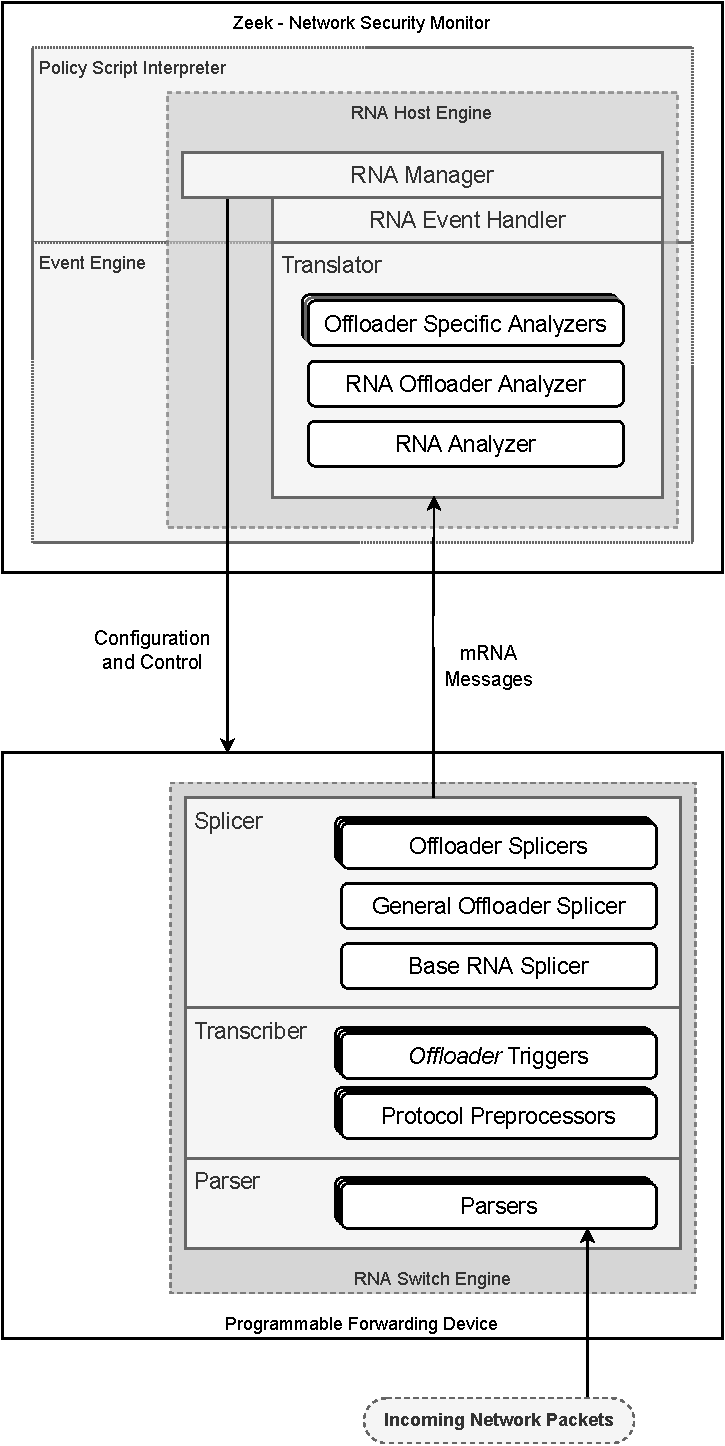
\includegraphics[width=0.7\textwidth]{images/arch_low_level.pdf}  
    \end{center}
    \label{fig:arch_low_level}
    \legend{Source: the author}
\end{figure}

\subsection{Switch Engine}

As the packet arrives at the P4-switch, it is first processed by the programmable parser. The \textbf{RNA Parser} component is a state machine with all the parsers the \Offloaders{} may need. Each one extracts its headers from the packet, and forwards the payload to the next parser.

In our example which is shown in Figure \ref{fig:icmp_ex_parser}, the first parser would be the Ethernet parser, extracting its header, followed by the IPv4 and ICMP parsers. In the example figure, we also display other states of parsers that were not identified. When the Ethernet header is parsed, the next protocol is defined by the \texttt{ethertype} field, which in this case was the IPv4 protocol. The states and protocols displayed by dotted lines were possible protocols the deployment could parse, but since the packet was an ICMP, those parsers were not used.

\begin{figure}[ht]
    \caption{Parsing States - ICMP Parsing Example}
    \begin{center}
        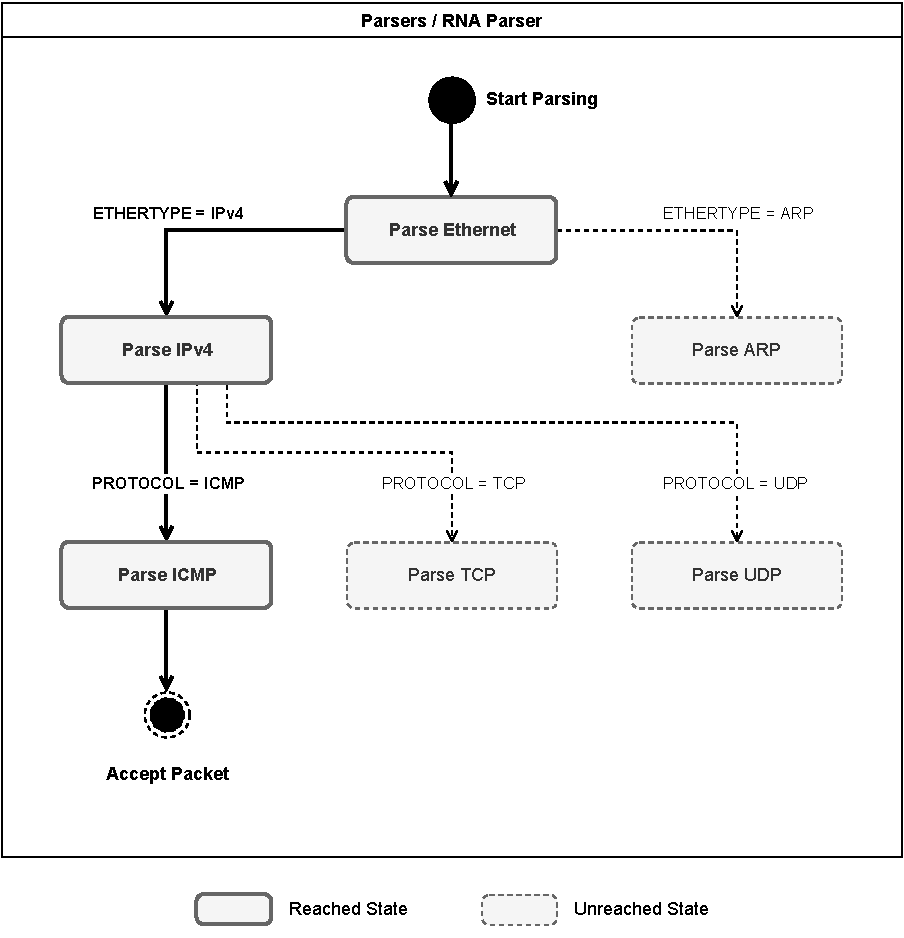
\includegraphics[width=0.7\textwidth]{images/icmp_ex_parser.pdf}  
    \end{center}
    \label{fig:icmp_ex_parser}
    \legend{Source: the author}
\end{figure}



The \textbf{RNA Transcriber} is the first component to be executed after the packets have their headers parsed, this happens in the ingress pipeline. In the Transcriber component, as shown in Figure \ref{fig:arch_low_level}, there are two types of modules, the Protocol Preprocessors and the Offloader Triggers, both of which may have multiple instances. We start explaining the Protocol Preprocessors since they are the first modules to be executed inside this component.

The Protocol Preprocessors are functions that every \ProtocolTemplate{} may execute to extract protocol metadata from the packet. This module is optional and every \ProtocolTemplate{} may have only one preprocessor. In our example, the processor extracts the ICMP type from the header and saves it in the metadata.

The next modules to be executed in the Transcriber are the Offloader Triggers, which are conditions that identify which \Offloader{} should be triggered. Each of these conditions is checked, and the first \Offloader{} to have its trigger condition valid is marked as the triggered one in the packet's metadata. In our example of an ICMP echo request, our trigger condition is \texttt{icmp.type = 8}. This ensures the \Offloader{} \textsc{ICMP Echo Request} is triggered when a ping packet arrives.

After a valid \Offloader{} is found, a copy of this packet is created and using this cloned packet, the switch will be able to construct the mRNA message. The original packet will follow its flow and be delivered to the originally intended destination. At this moment we transition into the Splicer component, where the construction of the summarized message starts. 

The \textbf{RNA Splicer} is executed after the packet leaves the ingress pipeline and it enters the egress pipeline\footnotemark{}. The RNA Splicer is composed of the two following types of splicers:

\begin{itemize}
    \item The \textbf{RNA Base Splicer} constructs the base header for the mRNA message. This header contains general information, which all \Offloaders{} can use. This includes, for example, source IP, destination IP, L3, and L4 protocols. In our example, the RNA Base Splicer sets both source and destination IPs, the L3 protocol to \texttt{IPv4}, and L4 protocol to \texttt{ICMP}. The Base Splicer is executed for every triggered \Offloader{}.
    
    \item The \textbf{Offloader Splicers} are splicers that every \Offloader{} may have. Each \Offloader{} Splicer constructs the header with the extra information required to execute its functionality. In our example, the \textsc{ICMP Echo Request} Splicer will construct a header with information about the ICMP packet: \texttt{type}, \texttt{code}, \texttt{sequence}, and \texttt{id}.
\end{itemize}

\footnotetext{Since we are explaining the architecture behind \TheSolutionName{}, we are not considering the inner workings of the programmable data plane, where a buffer connects the ingress and egress pipeline.}

After every Splicer has finished constructing their headers, the mRNA message will be ready. The payload and headers, which together form the mRNA, are then merged and sent to Zeek's monitoring interface, effectively finishing the processing on the Switch Engine. From now on, Zeek's Translators will work to support the monitoring infrastructure.

\subsection{Host Engine}

In the this section, we describe how the Host Engine receives the mRNA messages and uses them to execute the monitoring scripts. Figure \ref{fig:arch_low_level} shows the first components to receive the mRNA message are the Translators. In Zeek's architecture there is one module responsible for analyzing each protocol, which are called Analyzers. Every Analyzer parses their respective headers and forwards the payload to the next one.

The first Analyzer to receive the mRNA message is not displayed in Figure \ref{fig:arch_low_level} and is executed before the RNA Analyzer. Since the mRNA message is built over the Ethernet protocol, the first analyzer to receive the message is the Ethernet Analyzer. This Analyzer, using the \texttt{ethertype} code, forwards then every received packet to the Analyzer responsible for parsing the next protocol layer.




\section{Code Generation}
